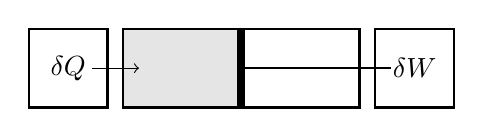
\begin{tikzpicture}[baseline=0.5cm]
  \def\sysLen{3};
  \def\sysHei{1};
  \def\sysDis{0.2};
  \def\syoLen{1};
  \def\filCol{white!90!black};
  \def\borDis{0.1};
  \def\ovrLap{0.2};

  \fill[\filCol] (0,0) rectangle (\sysLen/2,\sysHei);

  \draw[thick] (0,0) rectangle ++(\sysLen,\sysHei);

  \fill[black] (\sysLen/2-\borDis/2,0) rectangle ++(\borDis,\sysHei);

  \draw[thick] (-\sysDis-\syoLen,0) rectangle ++(\syoLen,\sysHei);

  \node at (-\sysDis-\syoLen/2,\sysHei/2) {$\delta Q$};

  \draw[thick] (\sysLen+\sysDis,0) rectangle ++(\syoLen,\sysHei);

  \node at (\sysLen+\sysDis+\syoLen/2,\sysHei/2) {$\delta W$};

  \draw[->] (-\sysDis-\ovrLap,\sysHei/2) to (\ovrLap,\sysHei/2);

  \draw[thick] (\sysLen/2,\sysHei/2) to (\sysLen+\sysDis+\ovrLap,\sysHei/2);

\end{tikzpicture}
